\input{header.tex}

\subject{V601}
\title{Franck-Hertz-Versuch}
\date{%
  Durchführung: 29.06.2021
  \hspace{3em}
  Abgabe: 06.07.2021
}

\begin{document}
\pagenumbering{arabic} % damit Seitenzahlen nicht roemisch sind

\maketitle
\thispagestyle{empty}
\tableofcontents
\newpage

\section{Theorie}
\label{sec:Theorie}

In diesem Versuch untersuchen wir den Energietransport zwischen 
zwei Wärmereservoiren, mit dem Ziel die Kenngrößen der 
eingesetzten Wärmepumpe zu ermitteln.

\subsection{Das Prinzip der Wärmepumpe}
Aus Beobachtung von Prozessen in der Natur kann man sagen, dass Wärmeenergie immer vom heißeren zum kälteren
Körper fließt. Durch externe (mechanische) Arbeit kann man diesen Fluß jedoch umkehren. \\
Dabei nimmt nach 
dem ersten Hauptsatz der Wärmelehre das wärmere Reservoir die Wärmeenergie $Q_1$ auf, welche sich aus der
vom kälteren Reservoir entnommenen Wärmemenge $Q_2$, sowie der aufgewandten Arbeit $A$ zusammen:
\begin{equation}
	Q_1 = Q_2 + A
	\label{eqn:waermemenge}
\end{equation}

Davon ausgehend lässt sich die Güteziffer der Wärmepumpe als der Quotient von abgegebener Wärme
und aufgewandter Arbeit definieren:
\begin{equation}
	\nu = \frac{Q_1}{A}
	\label{eqn:gueteziffer}
\end{equation}

Aus dem zweiten Hauptsatz der Thermodynamik lässt sich dabei eine weitere Beziehung herleiten:
Ändert sich die Temperatur zwischen den Reservoiren nicht, so besagt dieser, dass
die Summe der sogenannten 
reduzierten Wärmemengen $\int \frac{\symup{d}Q}{T}$ verschwindet. Dies bedeutet für uns
\begin{equation}
	\frac{Q_1}{T_1} - \frac{Q_2}{T_2} = 0.
	\label{eqn:reduzierte}
\end{equation}

Dabei muss jedoch beachtet werden, dass \eqref{eqn:reduzierte} nur für ideale reversible 
Prozesse gilt. Dies kann von der technischen Realisierung der Wärmepumpe natürlich nicht erreicht werden.
Für den realistischen, irreversiblen Fall gilt die Beziehung
\begin{equation}
	\frac{Q_1}{T_1} - \frac{Q_2}{T_2} > 0.
	\label{eqn:reduzreal}
\end{equation}

\subsection{Die Arbeitsweise der Wärmepumpe}

\subsection{Die Bestimmung der Kenngrößen einer realen
Wärmepumpe}

\subsubsection{Bestimmung der realen Güteziffer}
\subsubsection{Bestimmung des Massendurchsatzes}
\subsubsection{Bestimmung der mechanischen Kompressorleistung 
$N_\text{mech}$}

% \cite{sample}

\section{Durchführung}
\label{sec:Durchführung}
In der Durchführung des Versuchs wird zuerst eine Schaltung aufgebaut mit deren Hilfe die generelle Funktionsweise eines Lock-In-Verstärkers untersucht wird. Im zweiten Versuchsteil wird eine Photodetektorschaltung aufgebaut, mit der die Lichtintensität einer LED in Abhängigkeit des Abstandes zwischen  der LED und der genutzten Photodiode untersucht wird.
\subsection{Untersuchung der Funktionsweise eines Lock-In-Verstärkers}
Der schmatische Aufbau der genutzten Schaltung für die Untersuchung der Funktionsweise eines Lock-In-Verstärkers ist in \autoref{fig:schema2} dargestellt.
\begin{figure}[H]
    \centering
    \includegraphics{images/schema2.JPG}
    \caption{Schematischer Aufbau der Messschaltung zur Untersuchung der Funktionsweise eines Lock-In-Verstärkers. \cite{sample}}
    \label{fig:schema2}
\end{figure}
\noindent
Zur praktischen Realisierung der Schaltung aus \autoref{fig:schema2} wird die Apparatur aus \autoref{fig:app} genutzt. Dazu werden die Anschlüsse entsprechend \autoref{fig:schema2} verschaltet.
\begin{figure}[H]
    \centering
    \includegraphics{images/schaltung.JPG}
    \caption{Schaltapparatur für die Realisierung eines Lock-In-Verstärkers. \cite{sample}}
    \label{fig:app}
\end{figure}
\noindent
Im ersten Teil der Messung wird der Noise Generator nicht genutzt, damit die Abhängigkeit zwischen der Phase der Referenzspannung und der Ausgangsspannung untersucht werden kann. Dabei werden sieben Messwerte zu der Phase der Referenzspannung und der Ausgangsspannung notiert. \newline
Im Anschluss wird der Noise-Generator angeschaltet, um den Einfluss eines zusätzlichen Rauschens auf die Spannung zu untersuchen. Dazu wird auf dem Oszilloskop ein Bild der Spannung mit eingeschaltetem Noise-Generator und ein Bild ohne Noise-Generator aufgenommen. 
\subsection{Photodetektorschaltung}
Für die Untersuchung der Lichtintensität der genutzten LED wird eine Photodetektorschaltung nach \autoref{fig:photo} aufgebaut.
\begin{figure}[H]
    \centering
    \includegraphics{images/photo.JPG}
    \caption{Schematischer Aufbau der Photodetektorschaltung zur Untersuchung der Lichtintensität der LED. \cite{sample}}
    \label{fig:photo}
\end{figure}
\noindent
Bei dieser Schaltung wird dann der Abstand zwischen LED und Photodiode nach und nach variiert und dabei werden Messwerte von dem Abstand zwischen LED und Photodiode sowie der gemessenen Spannung notiert.
\section{Auswertung}
\label{sec:Auswertung}

\subsection{Untersuchung der Phasenabhänigkeit der Ausgangsspannung}
\label{sec:Untersuchung der Phasenabhänigkeit der Ausgangsspannung}
Im ersten Teil wurde der Zusammenhang zwischen Ausgangsspannung und der Phase der
Referenzspannung untersucht. Dabei wurden sieben Messwerte aufgenommen, welche in
\autoref{fig:plot1} dargestellt sind.
\begin{figure}
  \centering
  \includegraphics{phase.pdf}
  \caption{Messdaten und Curv Fit.}
  \label{fig:plot1}
\end{figure}


\section{Diskussion}
\label{sec:Diskussion}

\subsection{Diskussion der Phasenahängigkeit}
\label{sec:Diskussion der Phasenahängigkeit}
Im ersten Teil wurde der Zusammenhang zwischen Referenzphase und Amplitude untersucht. Die
Messdaten (\autoref{tab:messdaten-phase}) sind konsistent mit der Periodizitätsbedingung
\begin{equation}
	U(\phi) = U(\phi + 2\pi) \approx -U(\phi + \pi).
\end{equation}
Dies spiegelt sich auch im Fitparameter $b = 0,96\pm0,12 \approx 1$ wieder. Problematisch
stellte sich die Identifikation eines Cosinus dar. Fit- und Theoriekurve sind um einen
Phasenfaktor von $\Delta \phi \approx \pi/4$ verschoben. Dies lässt sich auf den
Koeffizient $c = 0,86 \pm 0,49 \approx \pi / 4$ schieben. Um aus dem Sinus der
Fitfunktion einen Cosinus zu erhalten wäre fast das doppelte $c_\text{Theo} = \pi/2 \approx
1,57$ nötig gewesen.
\\
Die Skalenfaktoren in y-Richtung $a$ und $d$ stimmen mit der optischen Beobachtung einer
geringen y-Verschiebung überrein. In den Fitparametern wird das durch das
Verhältniss der Parameter mit $d \ll b$ deutlich.
\\
Für eine exaktere Bestimmung wären mehr Messwerte nötig gewesen, wobei dann jedoch das
Aliasing problematisch werden würde.

\subsection{Diskussion zur Diodenintensität}
\label{sec:Diskussion zur Diodenintensität}
Im dritten Teil wurde der Abfall der Diodenintensität in Abhängigkeit von der
Beobachterdistanz $d$ untersucht. Dabei wurden die zwei Funktionen
\begin{equation}
	U(d) = = \frac{a}{d} + b,
	\qquad
	a = (637 \pm 51,2) \, \frac{\si{\volt}}{\si{\centi\meter}}
	\quad
	b = (-20,7 \pm 3,5) \, \si{\volt}
\end{equation}
und 
\begin{equation}
	g(d) = \frac{a^\prime}{d^2} + b^\prime
	\qquad
	a^\prime = (4988 \pm 147,4) \, \frac{\si{\volt}}{\si{\centi\meter}}
	\quad
	b^\prime = (-3 \pm 0,82) \, \si{\volt}
\end{equation}
berechnet. Optisch ist die zweite Kurve sehr viel näher an den Messwerten in
\autoref{fig:plot-diode} dran. Auch sind die relativen Unsicherheiten sehr viel kleiner.
Damit konnte die $1/x$-Gesetzmäßigkeit experimentell nicht bestätigt werden.
\\
Auffällig sind bei beiden Fits die Werte $b < b^\prime < 0$. Die entspräche einem Raum mit
negativem Untergrund, welcher offensichtlich nicht möglich ist. Die Messung sollte
wahrscheinlich unter besseren Bedingungen (Raum verdunkeln) durchgeführt werden, um
mögliche Fehlerquellen auszuschließen. 



\printbibliography{}

\appendix
\section{Anhang}
\label{sec:Anhang}

\begin{figure}
	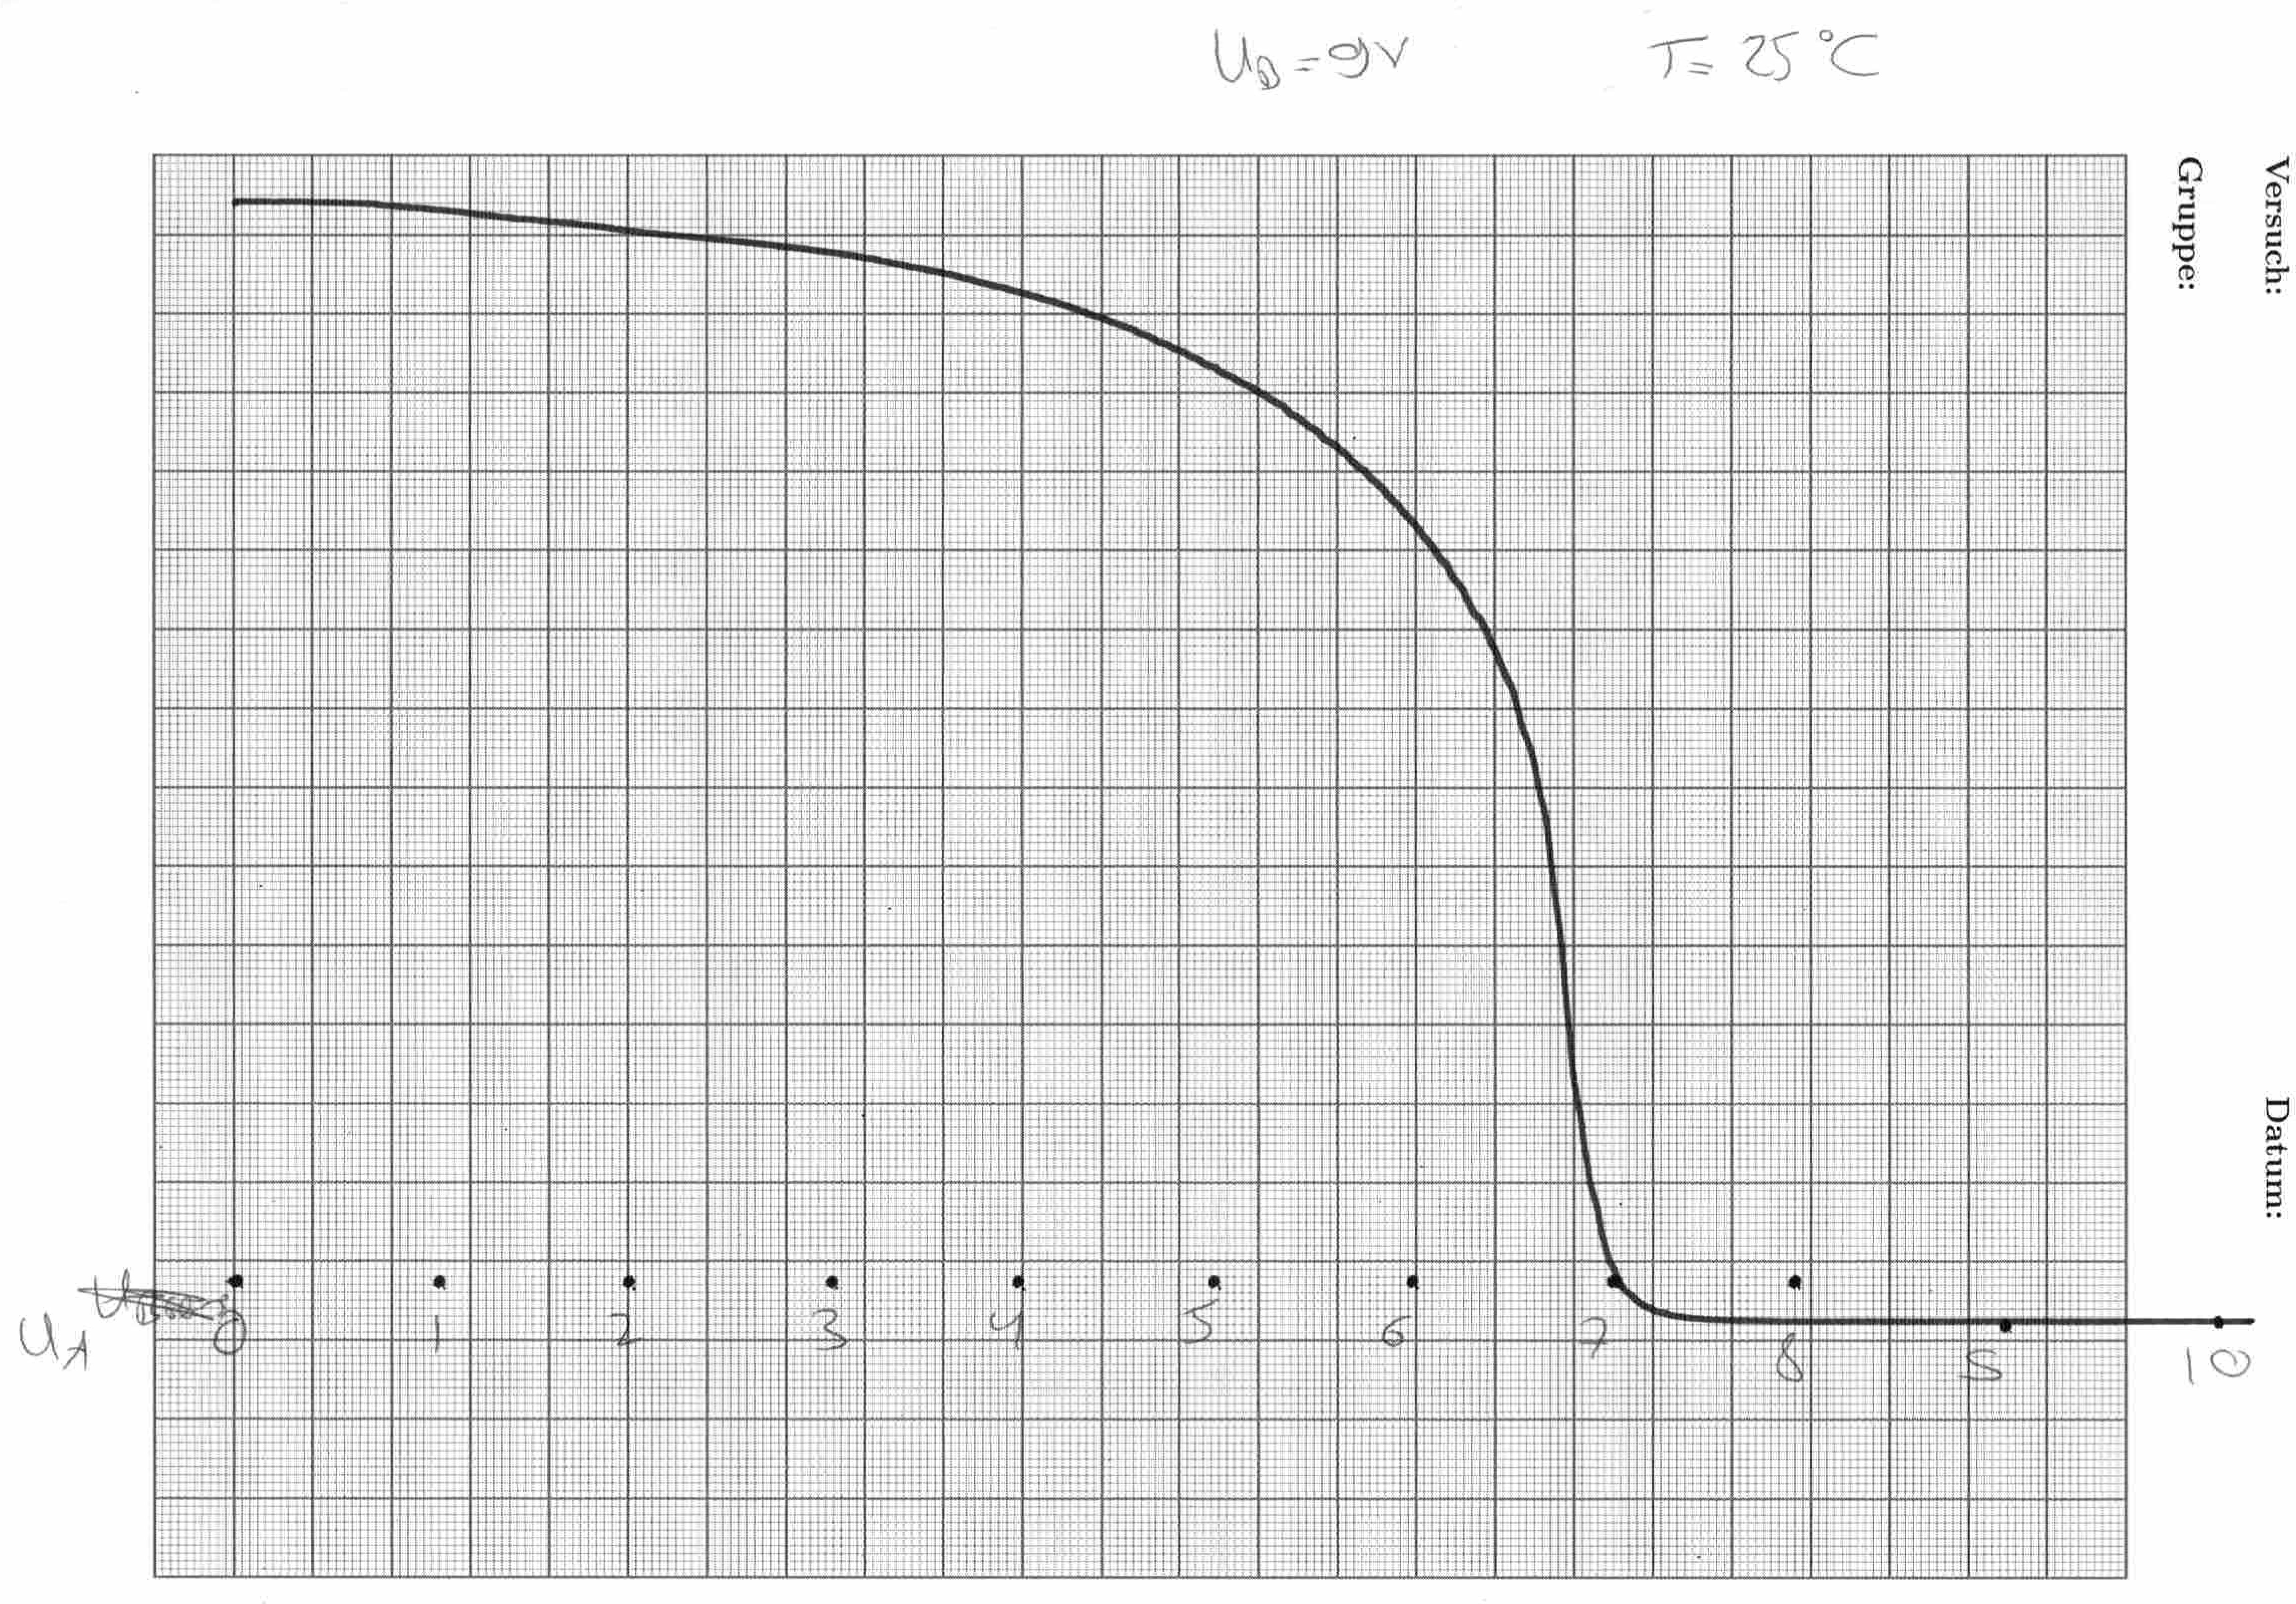
\includegraphics[width=0.8\textwidth]{Daten/0025.jpg}
	\caption{Original Messdaten zu $\SI{25}{\celsius}$.}
\end{figure}
\begin{figure}
	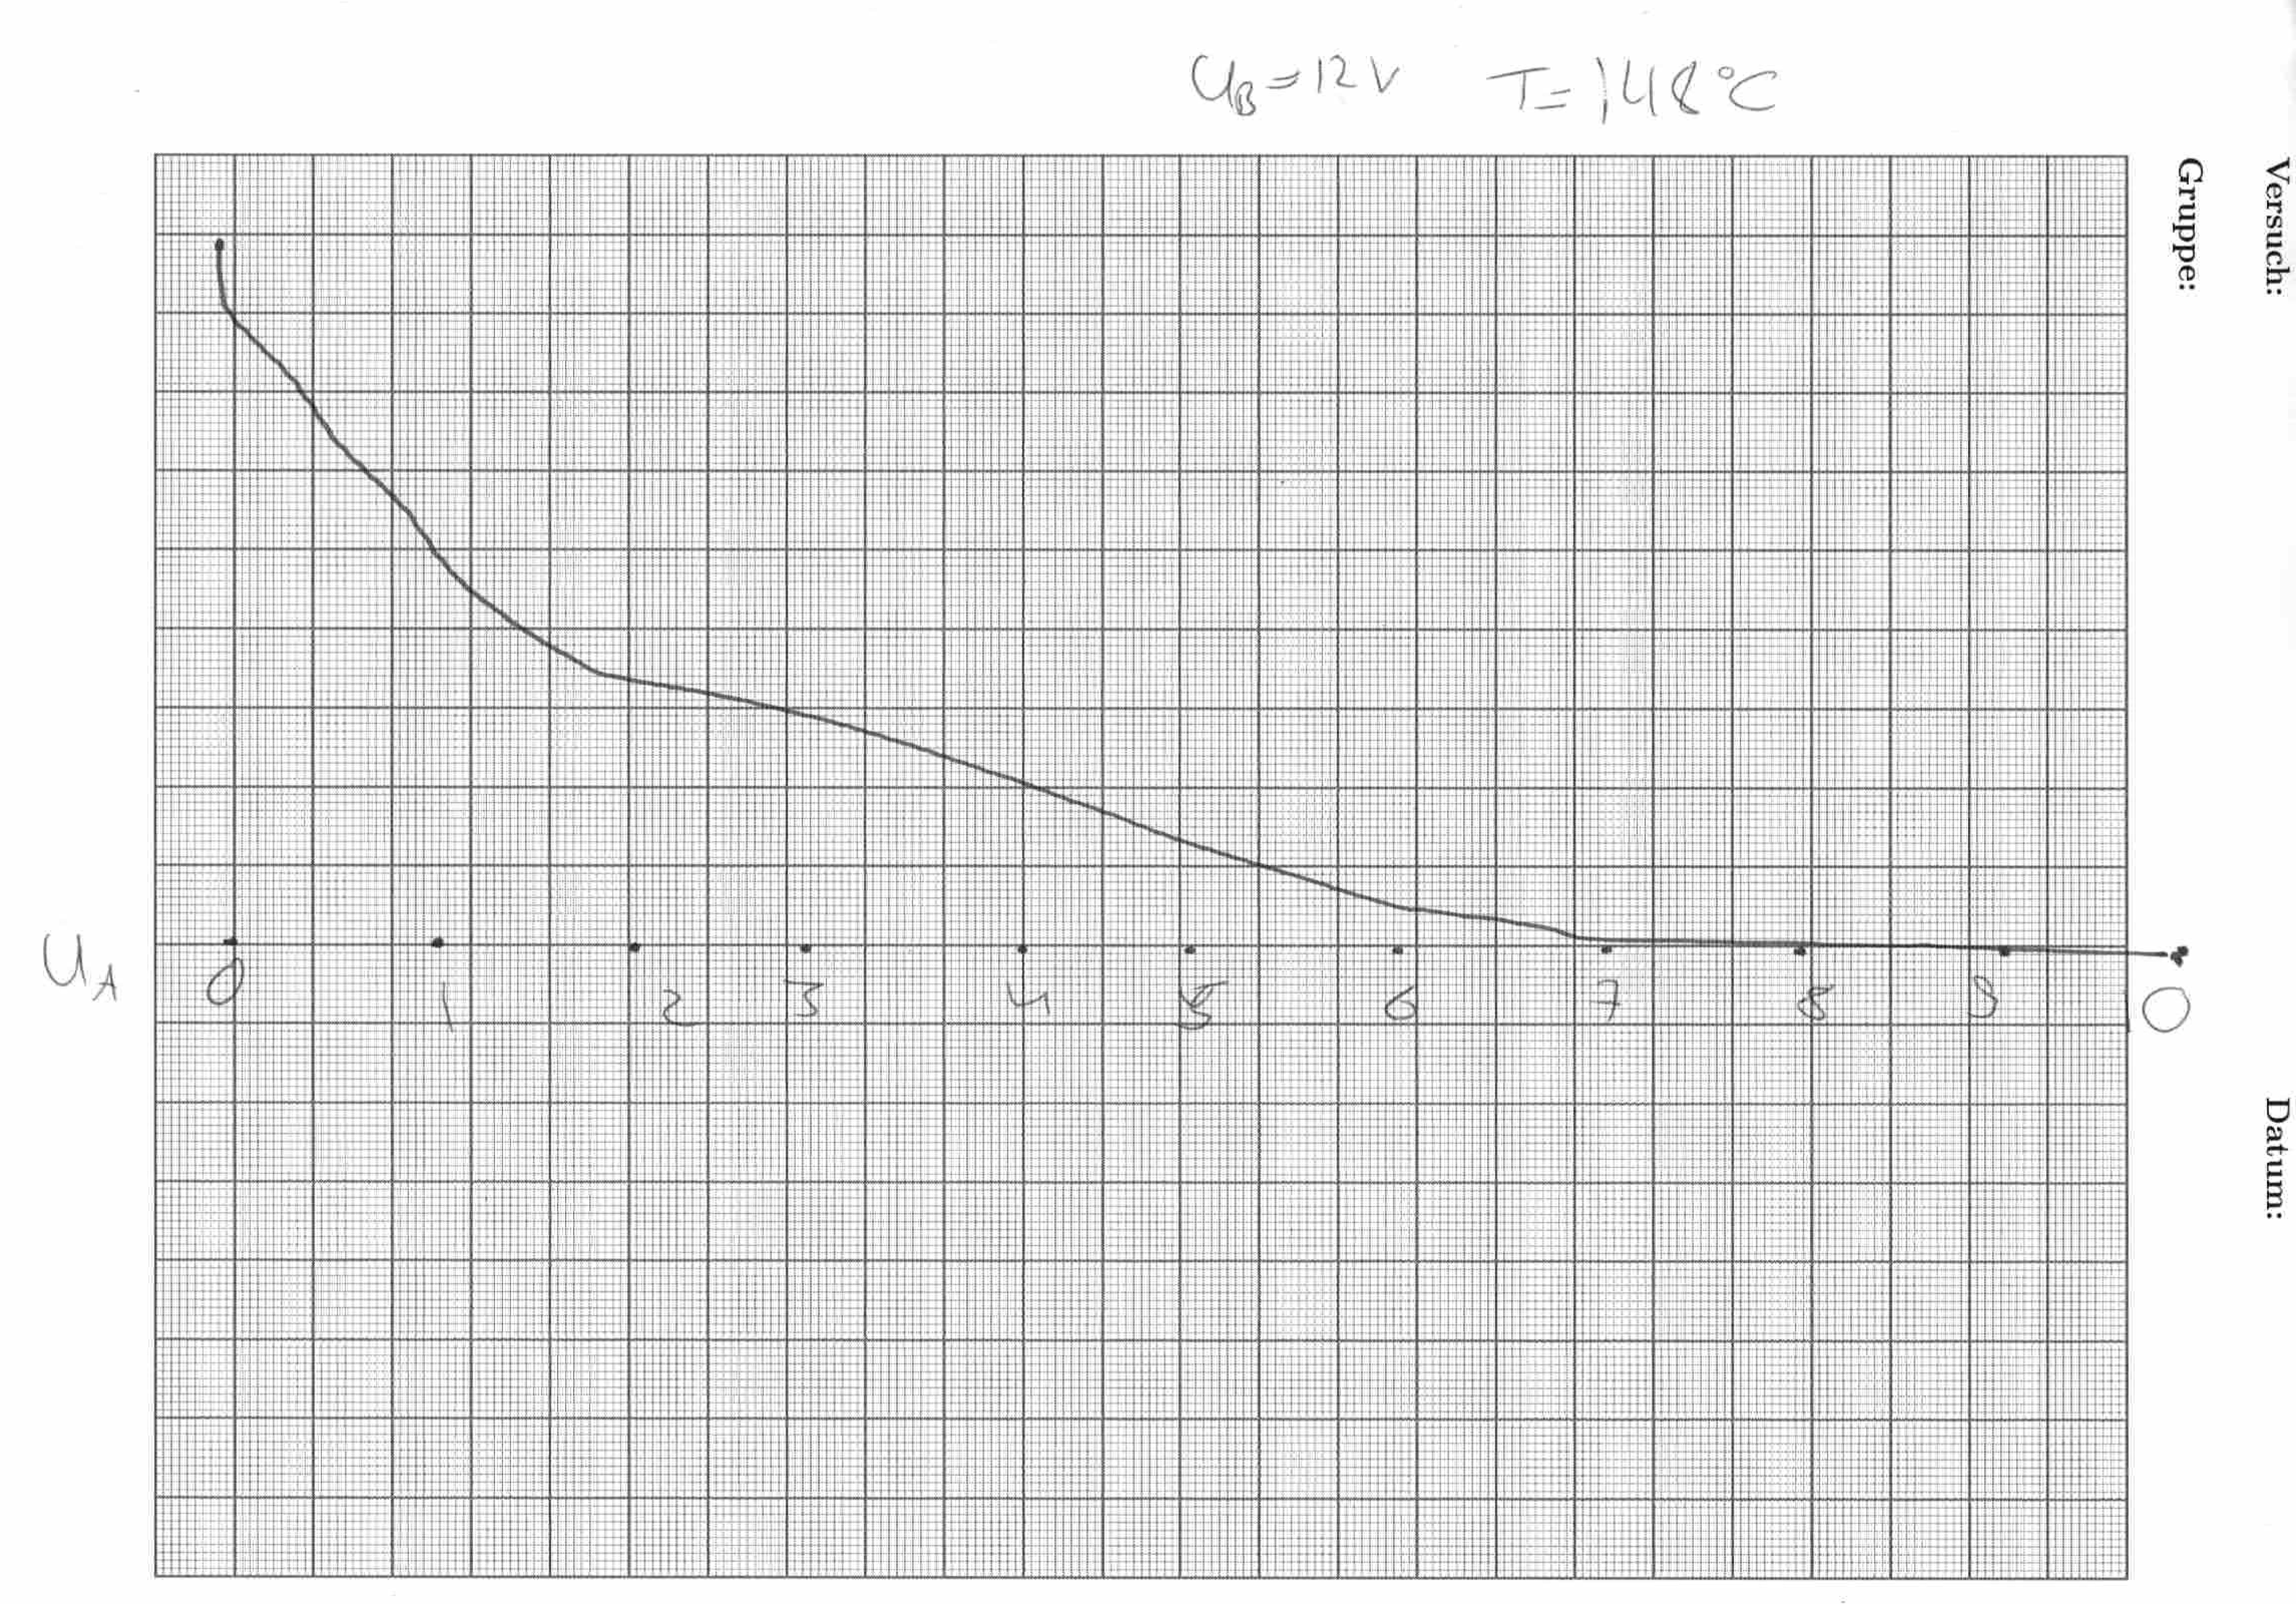
\includegraphics[width=0.8\textwidth]{Daten/1480.jpg}
	\caption{Original Messdaten zu $\SI{148}{\celsius}$.}
\end{figure}
\begin{figure}
	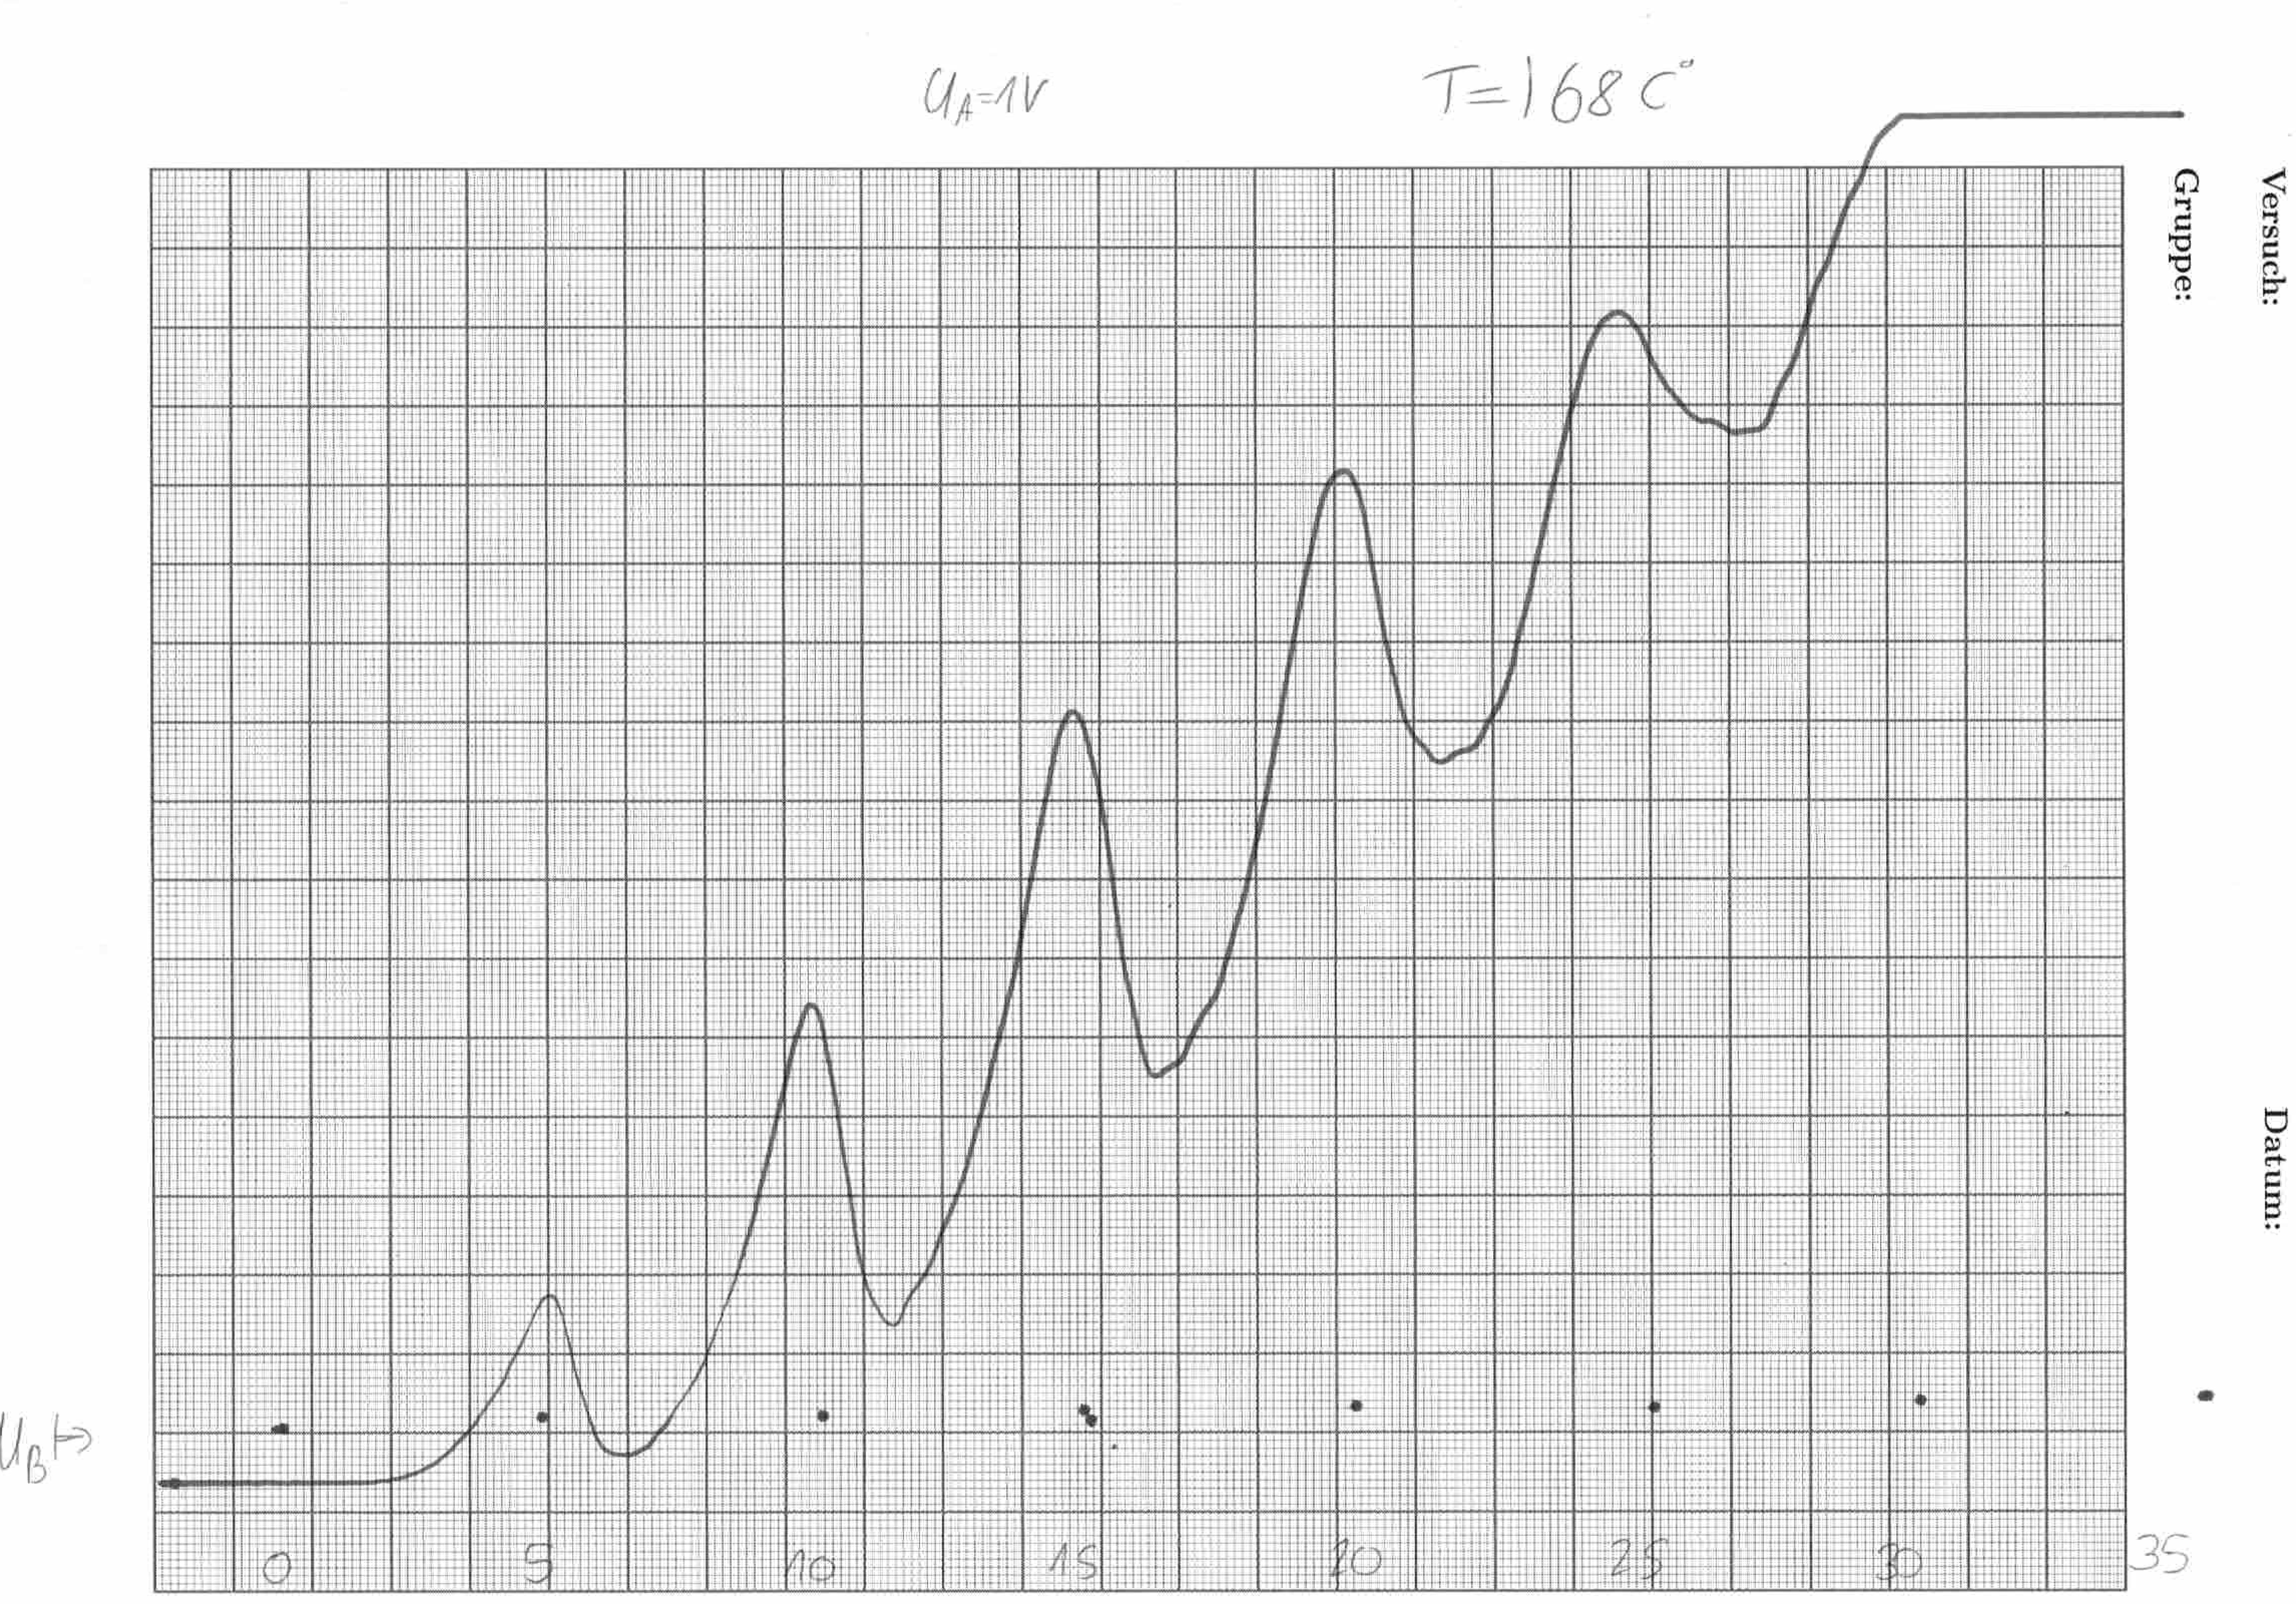
\includegraphics[width=0.8\textwidth]{Daten/1680.jpg}
	\caption{Original Messdaten zu $\SI{168}{\celsius}$.}
\end{figure}
\begin{figure}
	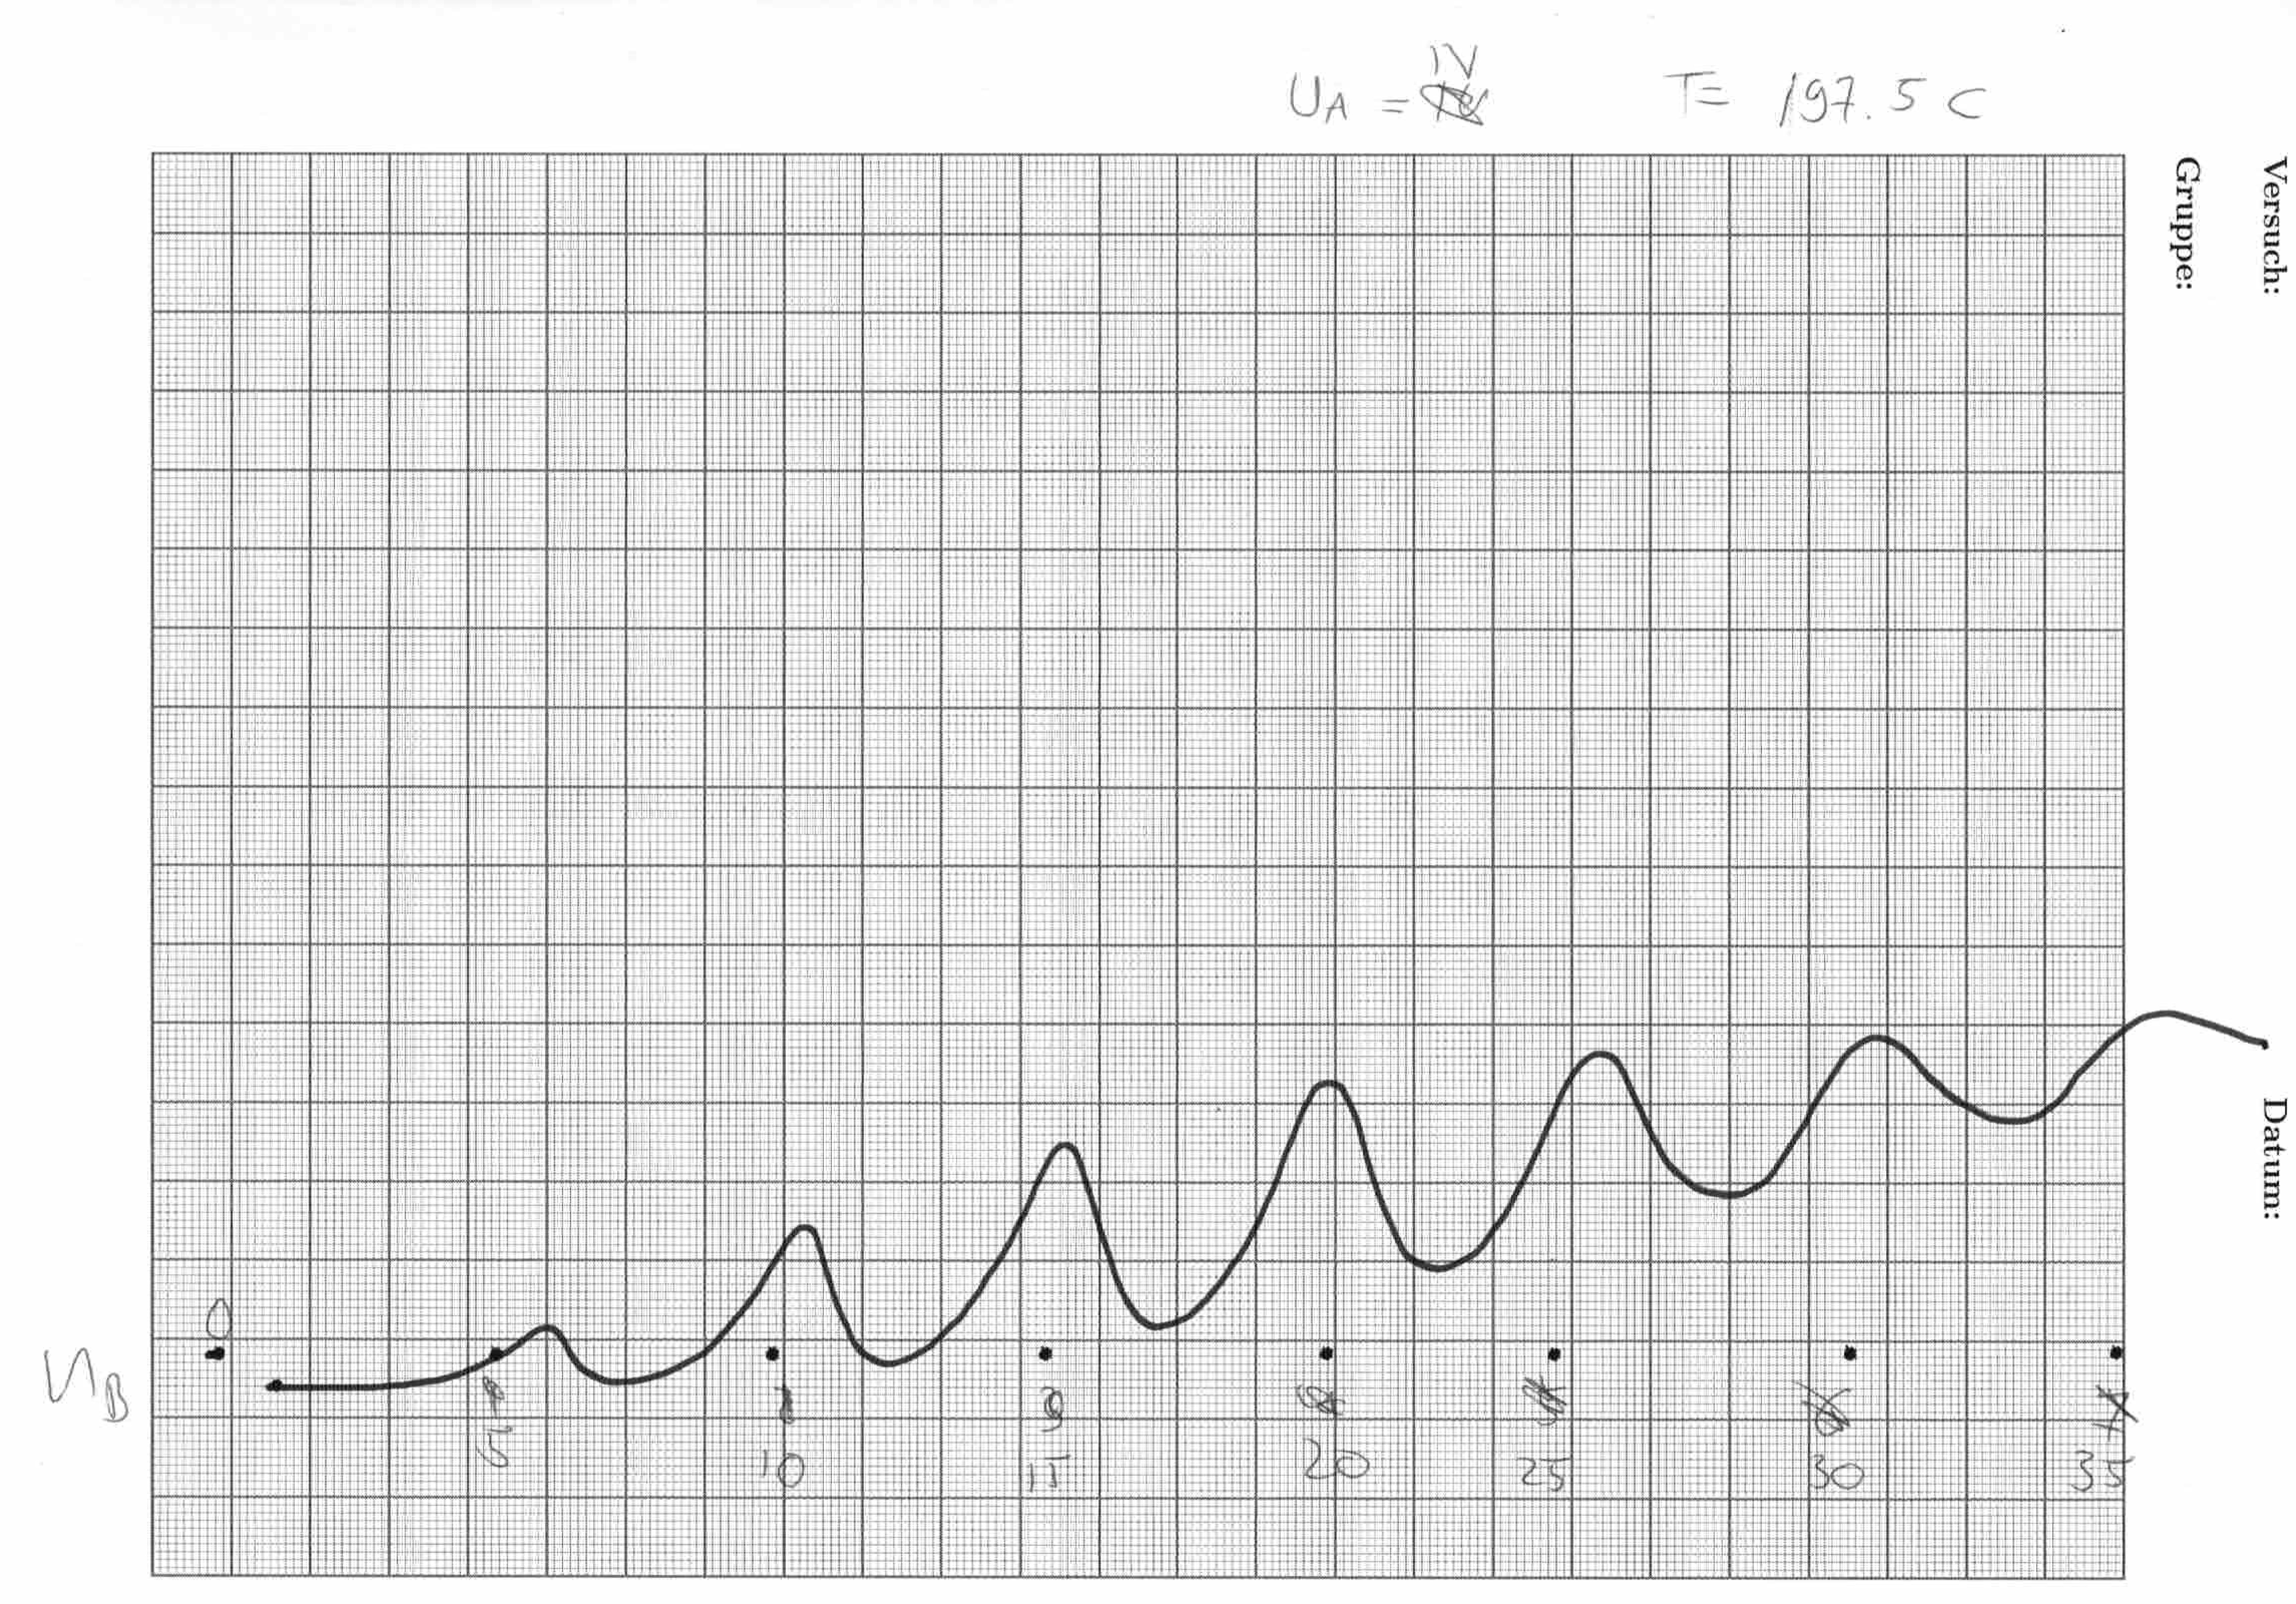
\includegraphics[width=0.8\textwidth]{Daten/1975.jpg}
	\caption{Original Messdaten zu $\SI{197.5}{\celsius}$.}
\end{figure}

\end{document}
